%%%%%%%%%%%%%%%%%%%%%  preambulo%%%%%%%%%%%%%%%%%%
\documentclass{article}

%%%%%%  paquetes%%%%
\usepackage{amsmath}   % Permite manipulacion de ecuaciones matematicas  
\usepackage{graphicx}  % Permite incluir graficos
\usepackage[spanish]{babel}   % Para establecer idioma del doc.
\usepackage[utf8x]{inputenc}  % Para incluir las tildes.

%%%%%% variables %%%%
\title{Ejemplo de documento realizado usando Latex}
\author{Leon Diaz}

%%%%%%%%%%%%%%%%  cuerpo del documento%%%%%%%%%%%%%
\begin{document}
	
	\maketitle
	
	% llamando el entorno de abstract para incluir un resumen del documento
	\begin{abstract}
		En este pequeño documento tipo articulo mostramos algunos ejemplos de ecuaciones en Latex, asi como inclusión de gráficos y llamado de referencias bibliográficas.
	\end{abstract}
	
	
	\section{Ecuaciones con sumatorias, derivadas e integrales}
	En las siguientes ecuaciones asumimos que $\alpha$ y $\beta$ son numeros reales:
	Ecuación con sumatorias:
	\begin{equation}\label{ecuacion1}
	f(n) = \sum_{n=1}^{\infty} \alpha n^2   
	\end{equation} 
	
	Ecuación con derivadas:
	\begin{equation}\label{ecuacion2}
	\dfrac{\partial  y}{\partial x } + y = x^3
	\end{equation} 
	
	Ecuación con integrales:
	\begin{equation}\label{ecuacion3}
	\int_{a}^{b} f(x) dx  = F(b)-F(a)
	\end{equation} 
	
	Problema: resuelva las ecuaciones  \ref{ecuacion1}, \ref{ecuacion2} y \ref{ecuacion3}.
	
	\section{Sub-ambientes matemáticos}
	El sub-ambiente \texttt{split} sirve para dividir ecuaciones muy largas o escribir procedimientos:
	\begin{equation} 
	\begin{split} %sub-entorno para dividir ecuaciones 
	A(x) & = \frac{\pi x^2}{2} \\
	& = \frac{1}{2} \pi x^2
	\end{split}
	\end{equation}
	
	El sub-ambiente \texttt{pmatrix} sirve para escribir matrices y vectores
	\begin{equation} 
	\begin{pmatrix} %sub-entorno para incluir matrices
	1 & 2 & 3\\
	\beta & \alpha & 0
	\end{pmatrix} 
	\end{equation} 
	
	
	
	
	\section{Inclusión de gráfico}
	A continuación incluimos un grafico:
	
	%----------Incluyendo grafico en ambiente figura-----------%
	\begin{figure}[h]
		\centering
		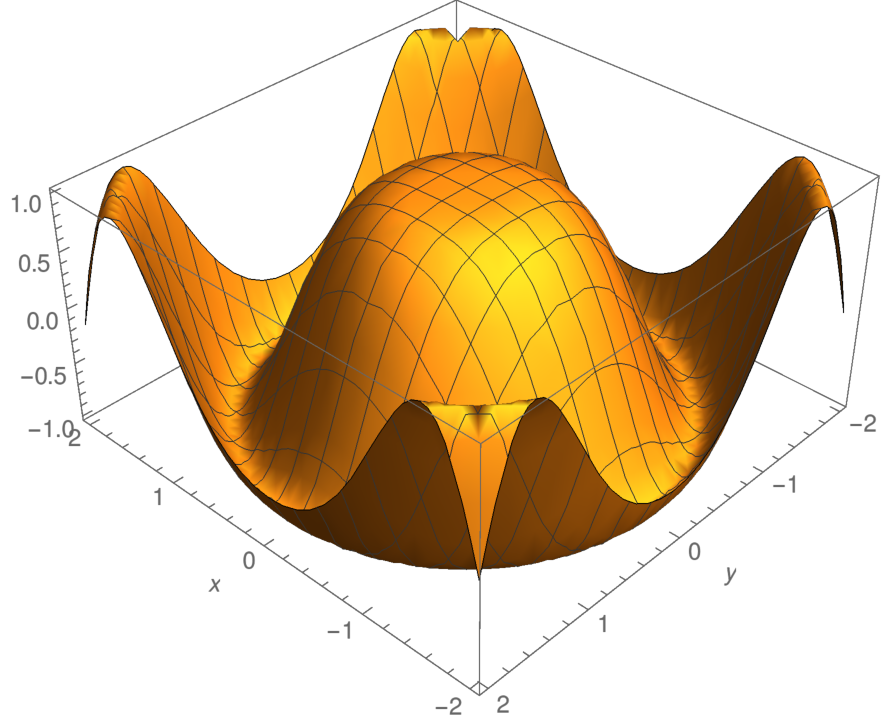
\includegraphics[scale=0.5]{imagen.pdf}
		\caption{Gráfico de la función $z=\cos ( x^2 + y^2 )$.}
		\label{etiquetadelgrafico}
	\end{figure}
	%----------------------------------------------------------%
	
	
	\section{Llamando una referencia bibliográfica}
	Para poder comprender el significado de la ecuación de campo de Einstein 
	
	\begin{equation*}
	R_{\mu \nu} - \dfrac{R}{2} g_{\mu \nu } = \kappa T_{\mu \nu}
	\end{equation*}
	
	sugerimos al lector ver \cite{einstein}. Adicionalmente, para hacer un programa 
	numérico que resuelva esta ecuación tensoria utilizando el lenguaje de
	programación Python consultar \cite{python}.
	
	
	%-----------el entorno de la bibliografía------------
	\begin{thebibliography}{99}
		
		%-----primera referencia--------
		\bibitem{einstein}{ 
			Albert Einstein. \textit{Zur Elektrodynamik bewegter K\"orper}. Annalen der
			Physik, 322(10): 891-921, 1905.
		} 
		%--------------------------------
		
		
		%-----segunda referencia--------
		\bibitem{python}{ 
			Python official web site \texttt{https://www.python.org/}
		}
		%-------------------------------
		
	\end{thebibliography}
	
	
\end{document} 